\section{Fourier Series}
%-----------------Orthonormal functions--------------------%
\subsection{Orthonormal Functions}
\begin{itemize}
    \item \textbf{Orthonormal functions} has the following property:
    \[ 
        \langle \phi_{i}(t), \phi_{k}(t) \rangle = 
        \begin{cases}
        0, & i \neq k\\
        1, & i = k\\
        \end{cases} 
    \]
    where a set of $N$ signals $\{ \phi_{i}(t) \}_{i=1...N}$ with this property is referred to as an \textbf{orthonormal set of signals}.
    
    \textit{For example, the orthogonal unitary vectors ($\hat{\mathbf{e}}_x$, $\hat{\mathbf{e}}_y$, $\hat{\mathbf{e}}_z$) defining the coordinate axes ($i,j,k$) in a 3D Euclidean space.}

    \item Any signals in a given space can be described by the linear combination of the basis (orthonormal) signals,
    \[ x(t) = \sum_{i=1}^{N} a_{i} \phi_{i}(t) \]
    where $a_{i}$ are unknown complex or real numbers applied to each basis.
    
    \item The coefficients $a_{i}$ can be determined by projecting the signal into each function $\{ \phi_{i}(t)\}_{i=1...N} $:
    \begin{align*}
    \begin{split}
    \langle x(t), \phi_{k}(t) \rangle
    &= \langle \sum_{i=1}^{N} a_{i} \phi_{i}(t), \phi_{k}(t) \rangle \\
    &= \int_{-\infty}^{\infty} \sum_{i=1}^{N} a_{i} \ \phi_{i}(t) \ \phi_{k}^{*}(t) \mathrm{d}t\\
    &= \sum_{i=1}^{N} a_{i} \int_{-\infty}^{+\infty}\phi_{i}(t) \ \phi_{k}^{*}(t) \mathrm{d}t \\
    &= a_{k}
    \end{split} \end{align*}

    \begin{itemize}
        \item Scalar product is a linear operator.
        \item The coefficients provide all the information in the signal: if we know $a_{k}$, we know the signal.
        \item If the signal $x(t)$ belongs to a larger space, the projected signal will be an \textit{approximation} of the original signal with minimum MSE.
        \end{itemize} 
\end{itemize}

\begin{ex}{- Haar basis function}
Given the signal:
\[ \psi(t) = 
\begin{cases}
    1,      &   0 \leq t < \frac{1}{2}\\
    -1,     &   \frac{1}{2} < t \leq 1\\
    0,      &   \text{otherwise}\\
\end{cases} \]
The following signals define a set of orthonormal basis functions:
\[ 
    \psi_{rk} = \psi(2^{r}t-k) \ \text{for} \ r=0,1,2... \ \text{and} \ k=0,1,2,...,2^{r}-1 
\]

 \begin{figure}[H]
     \centering
     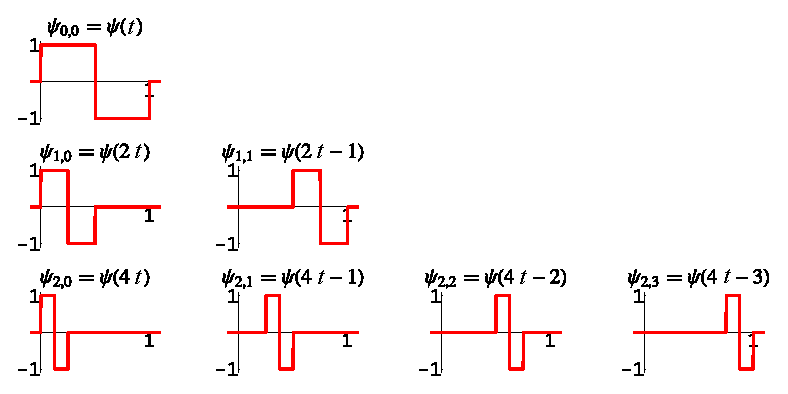
\includegraphics[width = \textwidth]{images/Haar_func.eps}
     \caption{Haar basis functions} 
 \end{figure}
\end{ex}
%-----------------Fourier basis functions--------------------%
\subsection{Fourier Basis Functions}
Fourier basis functions are:
\[
    \phi_{i}(t) = \frac{1}{\sqrt{T}} e^{j\omega_{i} t} =  \frac{1}{\sqrt{T}} e^{j\frac{2\pi\cdot i}{T} t} = \underbrace{\frac{1}{\sqrt{T}} \bigg[ \cos(\frac{2\pi \cdot i}{T} t) + j\sin(\frac{2\pi \cdot i}{T} t) \bigg]}_{\text{Euler's formula}},
\]
where $t$ is defined in the time interval $[0,T]$, $i \in \mathbb{Z}$ is an \textbf{integer}, and $j$ is the imaginary unit.\\

These functions have the following properties,
\begin{enumerate}
    \item periodic, the period is a function of the fundamental period $T$, $T_i= T/i$;
    \item the frequency of each Fourier basis function is an integer multiple of fundamental (base) frequency $\frac{1}{T}$;
    \item all basis functions are orthonormal to each other, when $0 \leq t \leq T$:
    \begin{itemize}
        \item if $i \neq k$, \textit{i.e.}, two distinguish basis functions,
        \[
            \langle \phi_{i}(t), \phi_{k}(t) \rangle = \int_{0}^{T}  \phi_{i}(t) \ \phi_{k}^{*}(t) \mathrm{d}t = \frac{1}{T} \int_{0}^{T} e^{j\frac{2\pi i}{T} t}e^{-j\frac{2\pi\cdot k}{T} t} \mathrm{d}t = 0,
        \]
        \item if $i=k$,
        \[
            \langle \phi_{i}(t), \phi_{k}(t) \rangle = \int_{0}^{T} \lvert \phi_{i}(t) \rvert^{2}\mathrm{d}t = \frac{1}{T} \int_{0}^{T}\mathrm{d}t =1
        \]
    \end{itemize}
\end{enumerate}

%-----------------Fourier Series-------------------%
\subsection{Fourier Series}
\textbf{Fourier series} can be used to represent any periodic signal with finite energy in a single period. 
\[
    x(t) =  \sum_{k=-\infty}^{\infty} \ c_{k} \ e^{j\frac{2\pi\cdot k}{T}t} \quad \text{with} \quad c_{k} = \frac{1}{T} \int_{-\frac{T}{2}}^{+\frac{T}{2}} x(t)e^{-j\frac{2\pi\cdot k}{T}t}
\]

\begin{dv}{}
    If we assume:
    \begin{align*}
    \begin{split}
        x(t) 
        &= \sum_{i=-\infty}^{+\infty} \ a_{i} \ \phi_{i}(t) \\
        &= \frac{1}{\sqrt{T}} \sum_{k=-\infty}^{+\infty} a_{k} \ e^{j\frac{2\pi\cdot k}{T}t}
    \end{split} 
    \end{align*}
    with the coefficients $a_{k}$ :
    \begin{align*}
    \begin{split}
        a_{k} = \langle x(t), \phi_{k}(t) \rangle 
        &= \int_{0}^{T} x(t)\ \phi_{k}^{*}(t)\mathrm{d}t \\
        &= \frac{1}{\sqrt{T}} \int_{0}^{T} x(t)\ e^{-j\frac{2\pi\cdot k}{T}t} \mathrm{d}t 
    \end{split}
    \end{align*}
    An equivalent expression is the \textbf{Fourier series}
    \[
        x(t) 
        = \sum_{k=-\infty}^{+\infty} \ c_{k} \ e^{j\frac{2\pi\cdot k}{T}t} 
        \quad \text{with} \ 
        c_{k} = \frac{1}{T} \int_{0}^{T} x(t)e^{-j\frac{2\pi\cdot k}{T}t} \mathrm{d}t
    \]
\end{dv}

\begin{itemize}
    \item The infinite set of orthonormal functions of the Fourier series describes any periodic signal with finite energy in a single period.
\end{itemize}

\begin{tcolorbox}[breakable]
Fourier series with a finite number of terms:
\[
    x(t) \approx x_{N}(t) = \sum_{k=-N}^{+N} c_{k} e^{j\frac{2\pi\cdot k}{T}t}
\]
The error of approximation decreases as the number of terms increases,
\[
    E_{N}(t) = x(t)-x_{N}(t) = x(t)- \sum_{k=-N}^{+N} c_{k} \ e^{j\frac{2\pi\cdot k}{T}t}
\]
\[
    \lim_{N \to \infty} \int_{0}^{T} \lvert E_{N}(t) \rvert^{2} \mathrm{d}t = 0, \quad \text{if} \ \int_{0}^{T} \lvert x(t) \rvert^{2} \mathrm{d}t < \infty
\] 
Fourier series converges as the number of terms increases:
\begin{figure}[H]
    \centering
    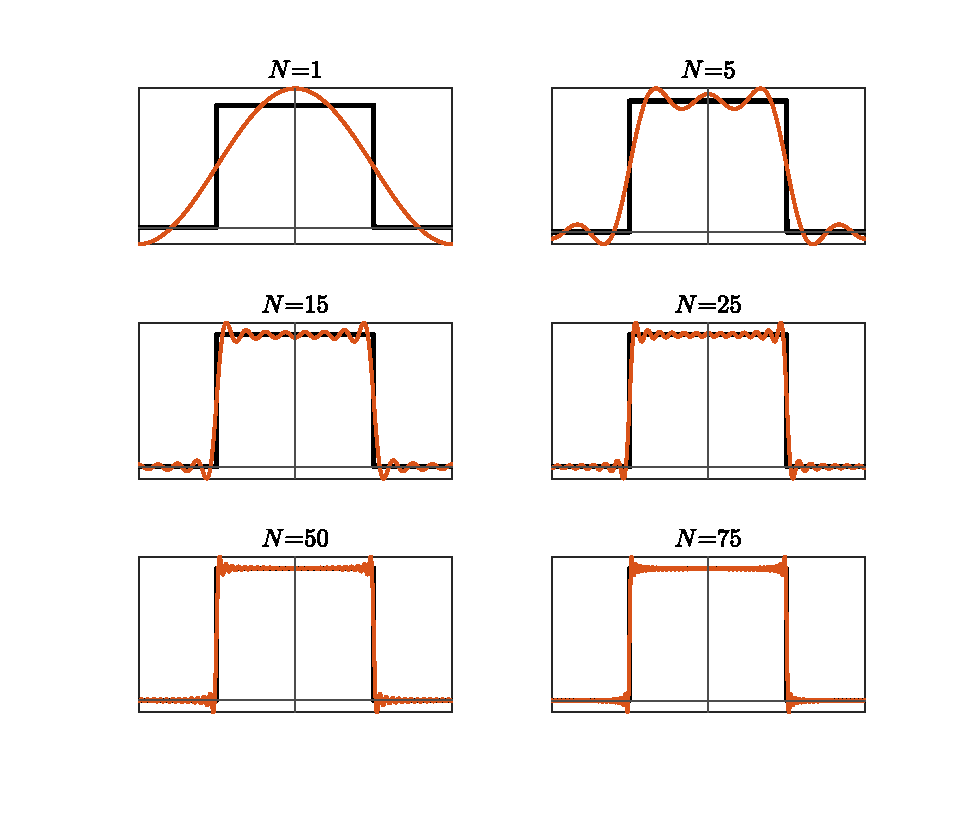
\includegraphics[width = \textwidth]{images/fSeries_terms.eps}
    \caption{Example of convergence of the Fourier series of a periodic square wave. Number of Fourier terms ($N$) increased from 1 to 75.} 
\end{figure}
\end{tcolorbox}
